\begin{quotation}
  {\footnotesize
    \noindent{\emph{``Most good programmers do programming not because they expect to get paid or get adulation by the public, but because it is fun to program.''\\}
    }
    \begin{flushright}
      Linus Torvalds
    \end{flushright}
  }
\end{quotation}
\vspace{0.5cm}

In this chapter the reader will first be presented with a qualitative analysis of the images produced with the toolbox illustrated in chapter \ref{chap:second-chapter}. After that, the preliminary validation of the \acrshort{svd} algorithm presented in chapter \ref{chap:third-chapter}  when applied to the same images will be discussed.

\section{Qualitative Assessment}
The aim of the toolbox presented in chapter \ref{chap:second-chapter} was to create batch of realistic images of a given CAD of a \acrshort{sc} in order to cope with the lack of an actual facility to produce images from a scale \acrshort{3d} printed model of the target itself, as done in \cite{Beierle2019}. The task of creating the toolbox itself was a tough one, but validating the goodness of the generated images is extremely difficult because of the actual lack of high-resolution and high-quality images taken in orbit by a real camera of a real \acrshort{sc}. So, the more realistic intent of this evaluation is therefore to compare the generated images to the SPEED\footnote{\url{https://kelvins.esa.int/satellite-pose-estimation-challenge/}}, in order to identify similarities and differences. As proposed in \cite{pangufinal}, the images can be compared in three ways:

\begin{itemize}
  \item visual comparison;
  \item image histogram comparison;
  \item basic feature extraction using a Sobel edge detector.
\end{itemize}

Unfortunately, the orbit and the true pose but more importantly the illumination conditions of each of the images contained in the SPEED data-set was not available at the time of writing this thesis, so it is impossible to present to the reader a one-to-one comparison. Still, it is worth to compare images which can be reasonably considered similar.

\begin{figure}[htbp]
  \centering
  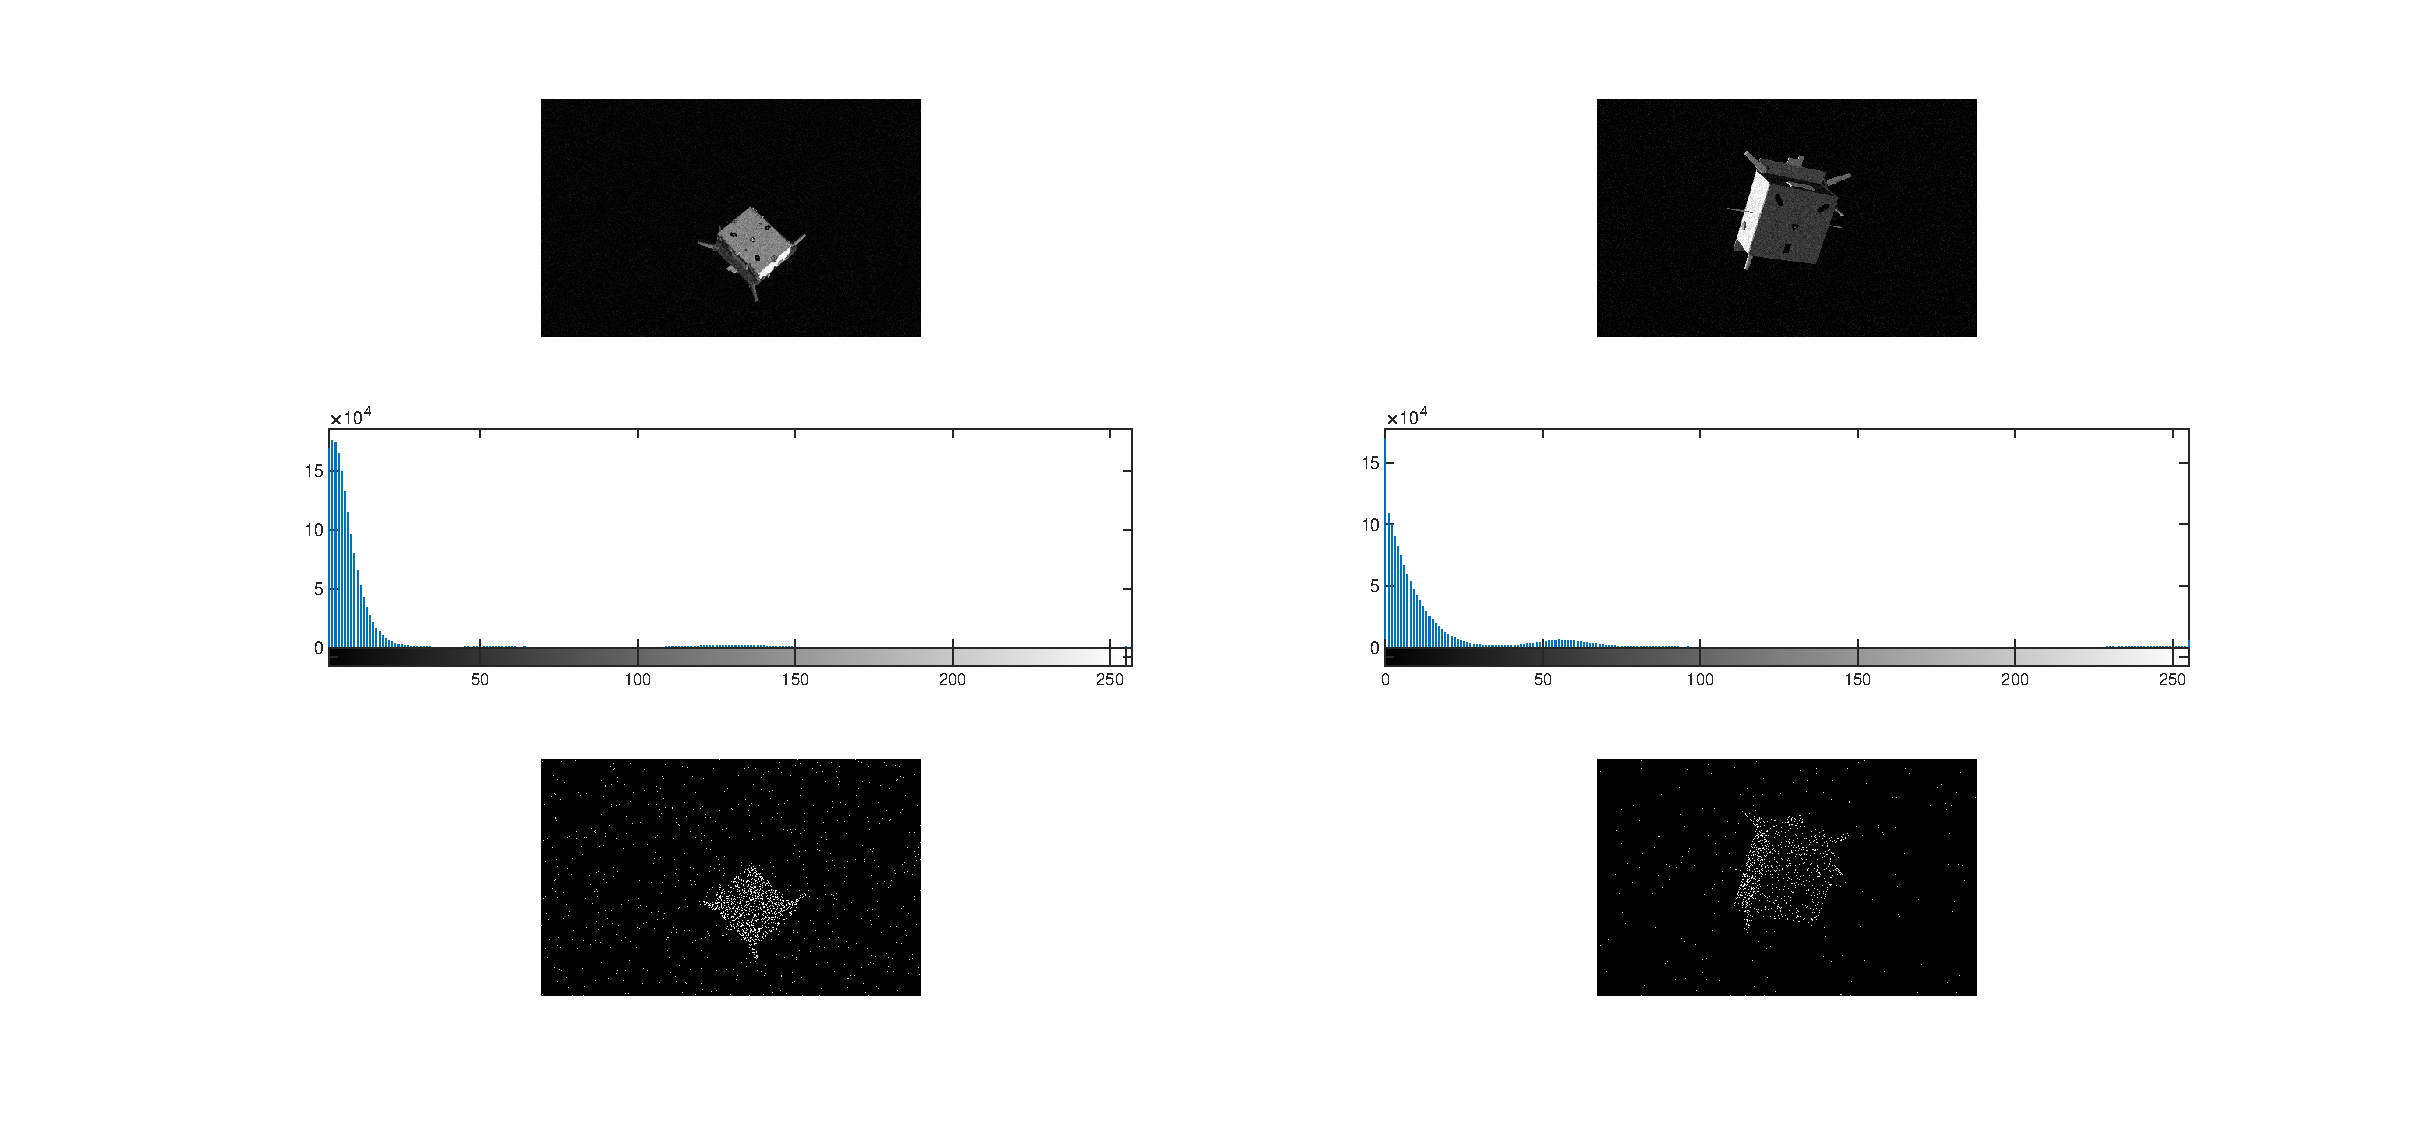
\includegraphics[width=1.0\textwidth]{gfx/comparison/comparison1.eps}
  \caption{Comparison between the SPEED data-set (left) and images generated using the toolbox presented in chapter \ref{chap:second-chapter} (right), 1}
  \label{fig:comparison1}
\end{figure}

\begin{figure}[htbp]
  \centering
  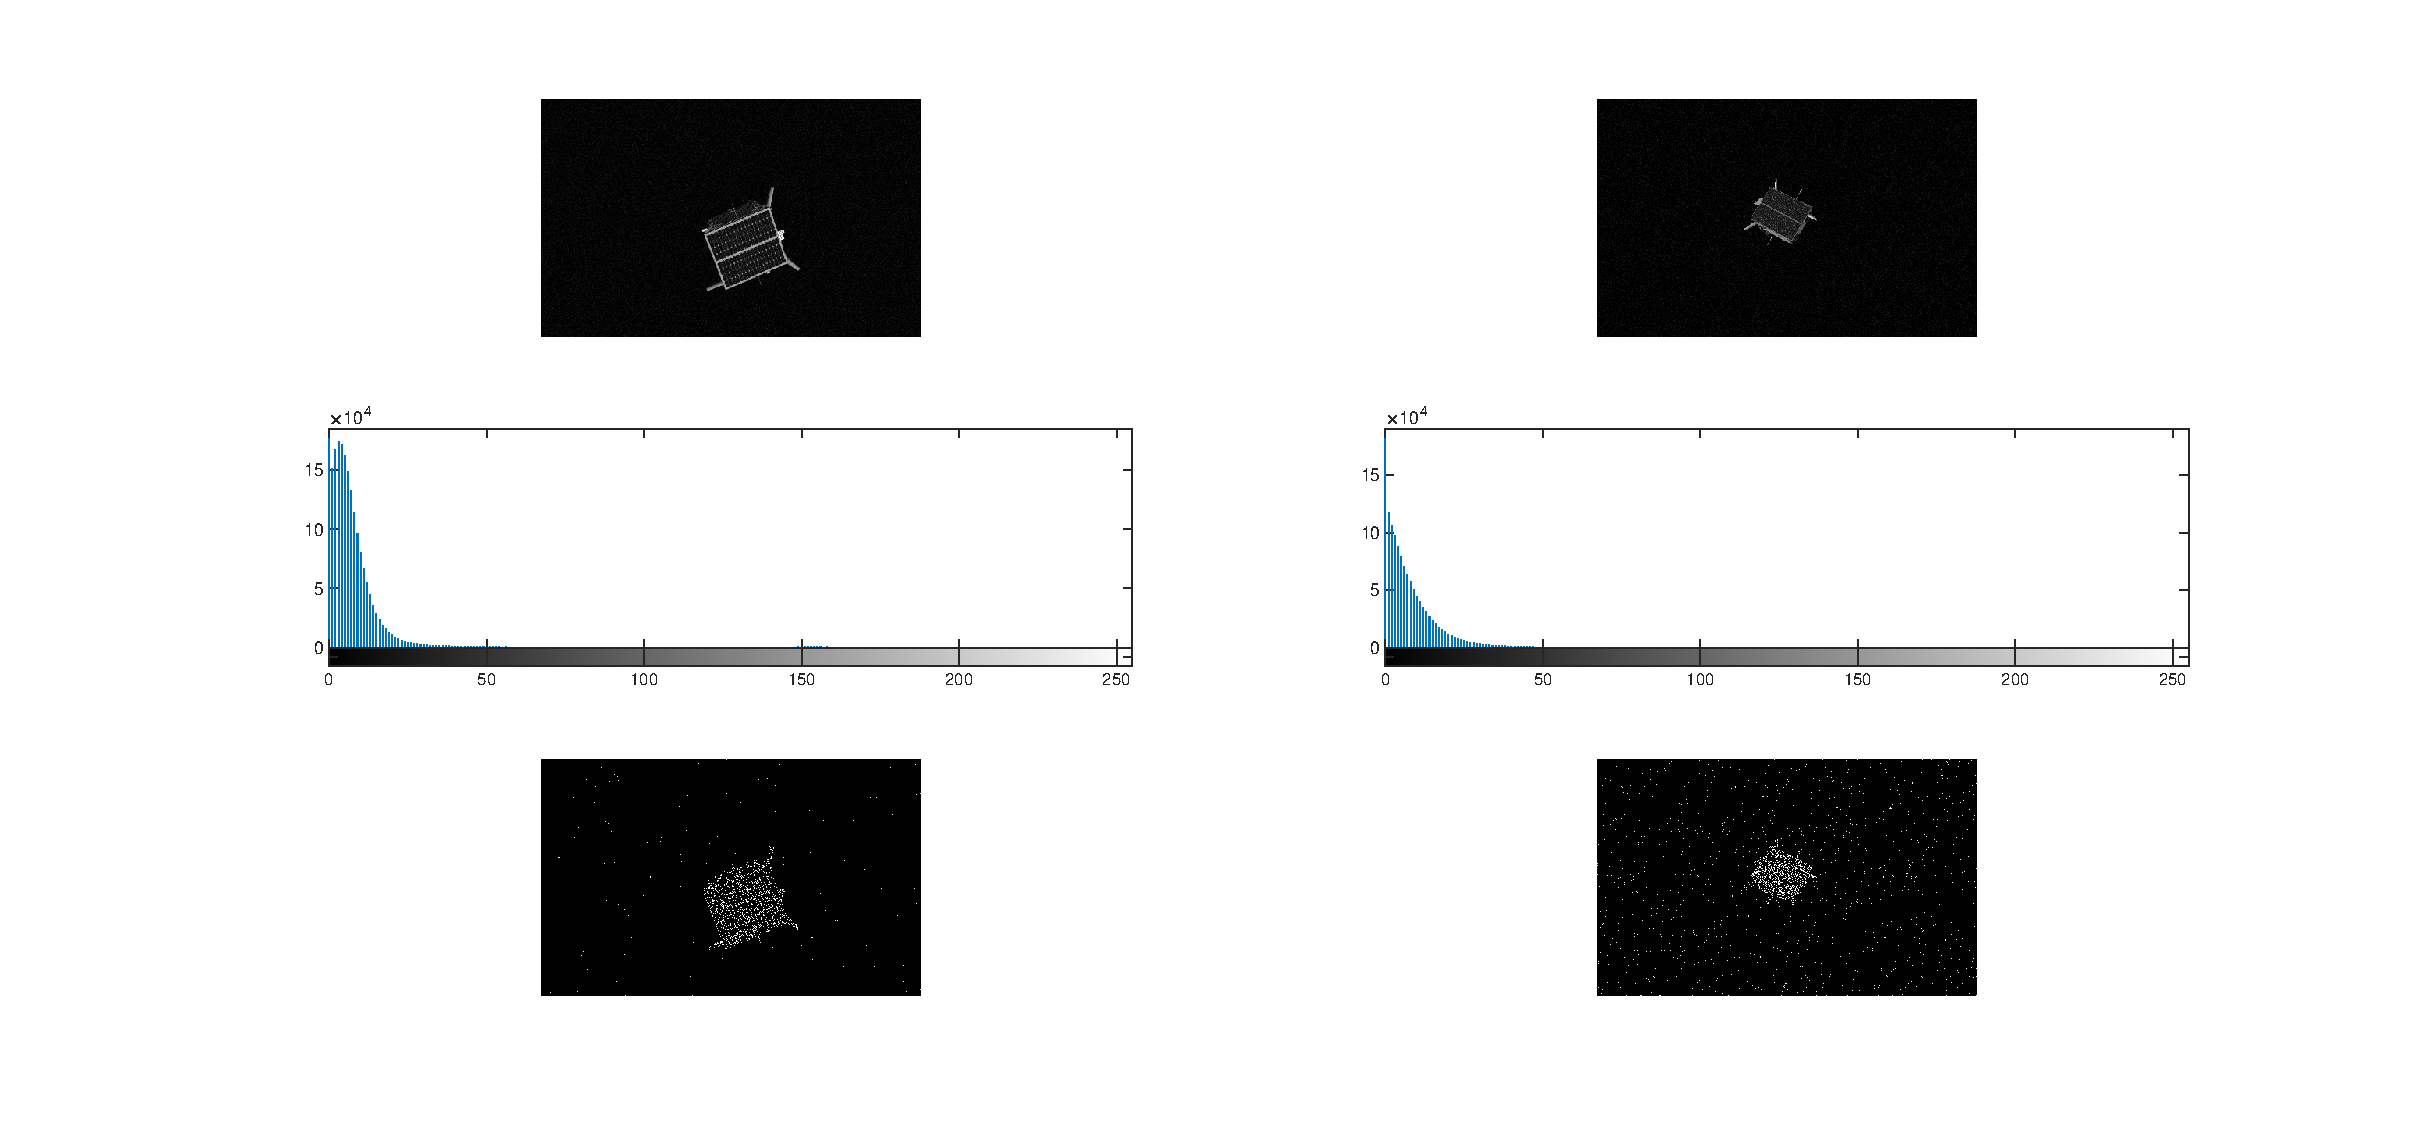
\includegraphics[width=1.0\textwidth]{gfx/comparison/comparison2.eps}
  \caption{Comparison between the SPEED data-set (left) and images generated using the toolbox presented in chapter \ref{chap:second-chapter} (right), 2}
  \label{fig:comparison2}
\end{figure}

\begin{figure}[htbp]
  \centering
  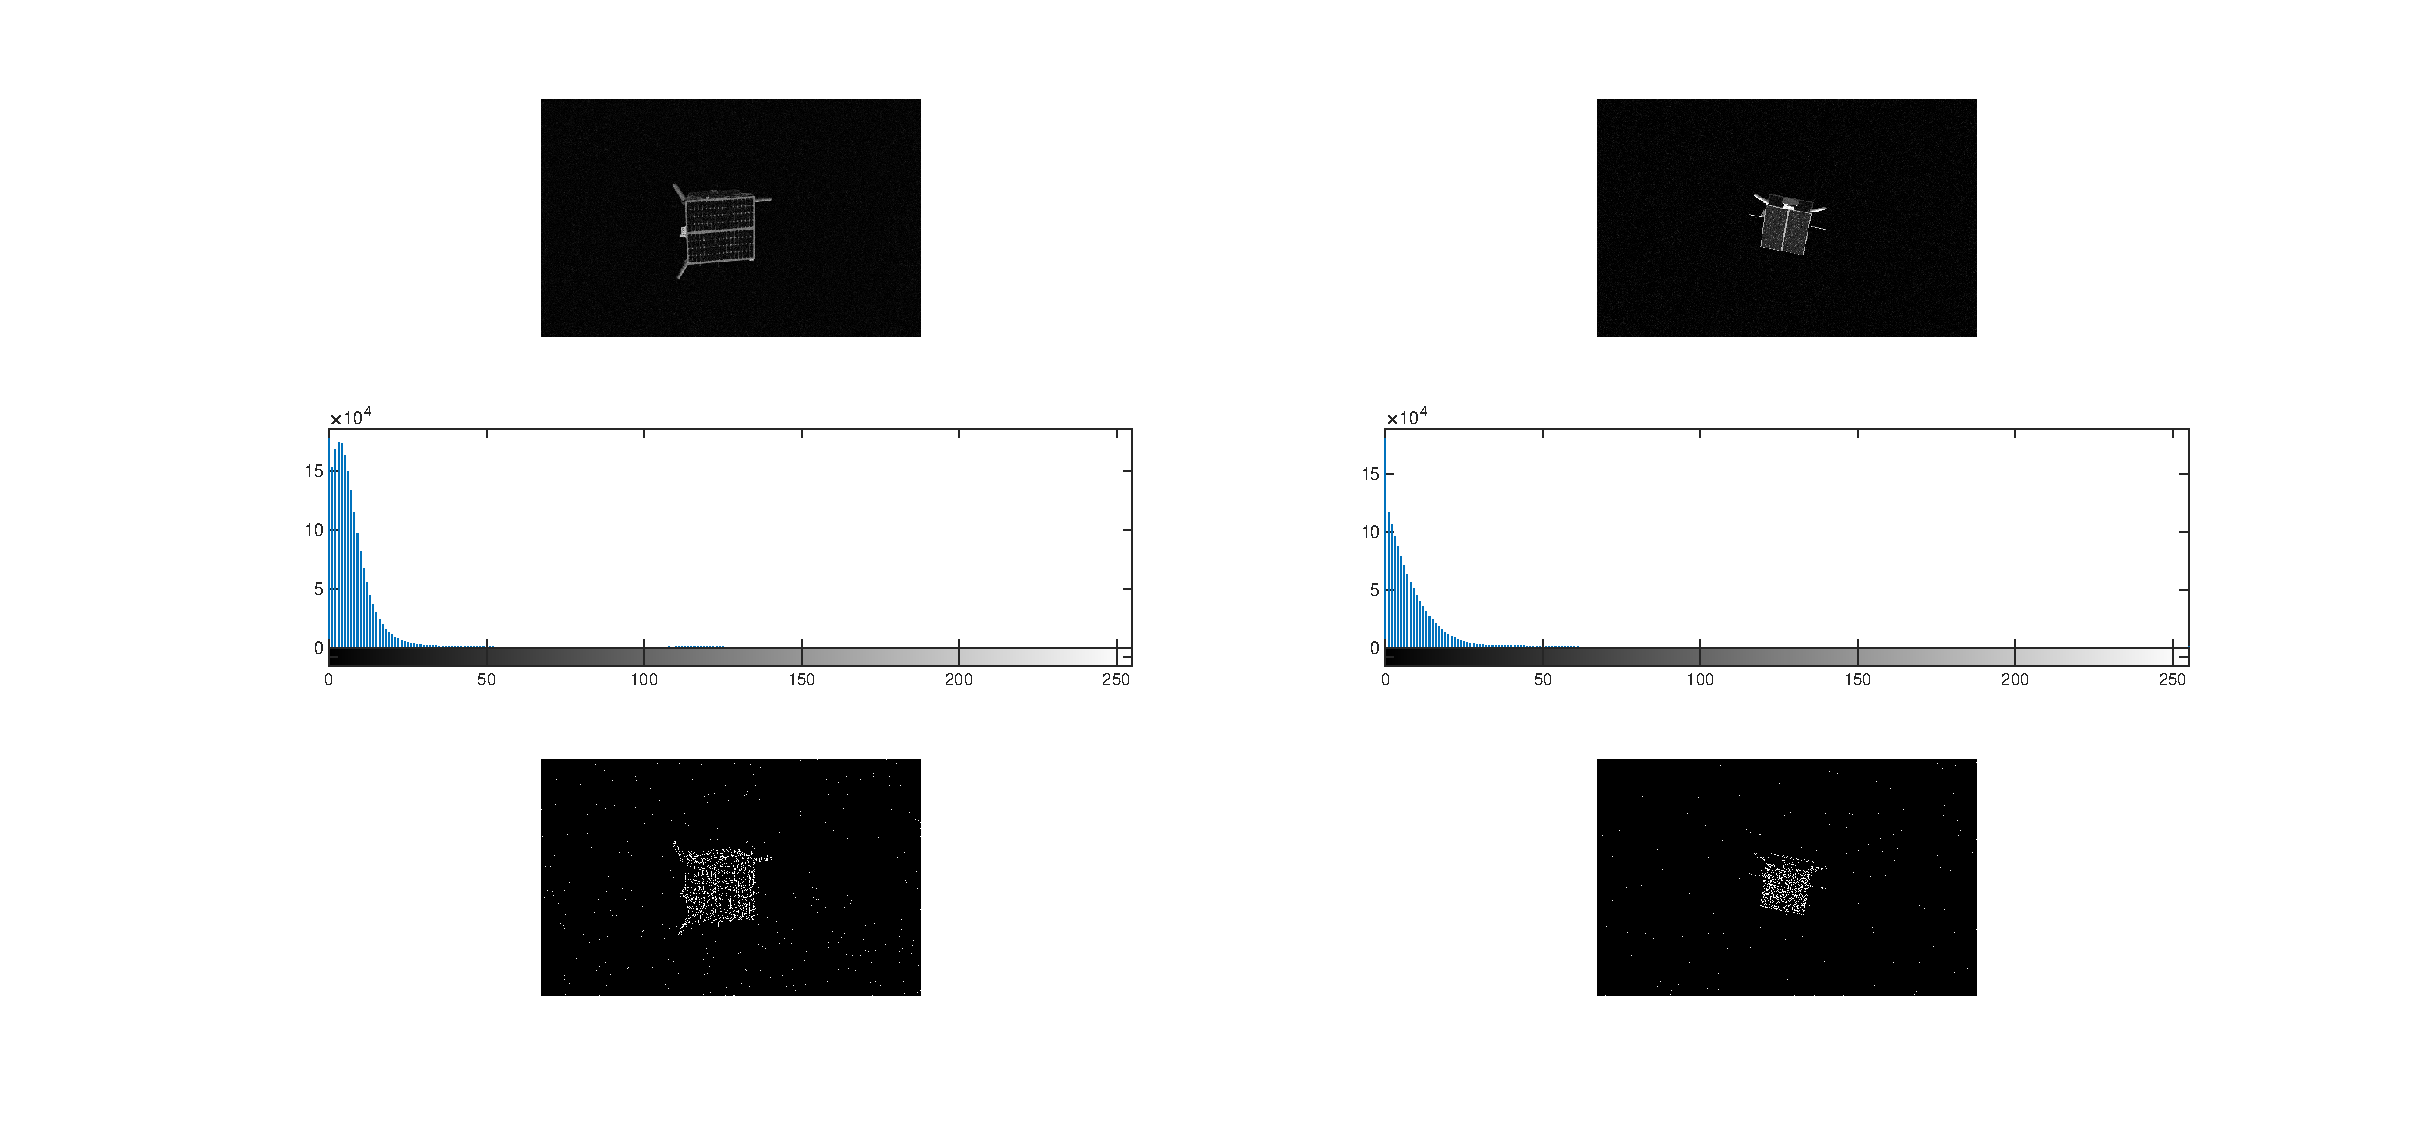
\includegraphics[width=1.0\textwidth]{gfx/comparison/comparison3.eps}
  \caption{Comparison between the SPEED data-set (left) and images generated using the toolbox presented in chapter \ref{chap:second-chapter} (right), 3}
  \label{fig:comparison3}
\end{figure}

\begin{figure}[htbp]
  \centering
  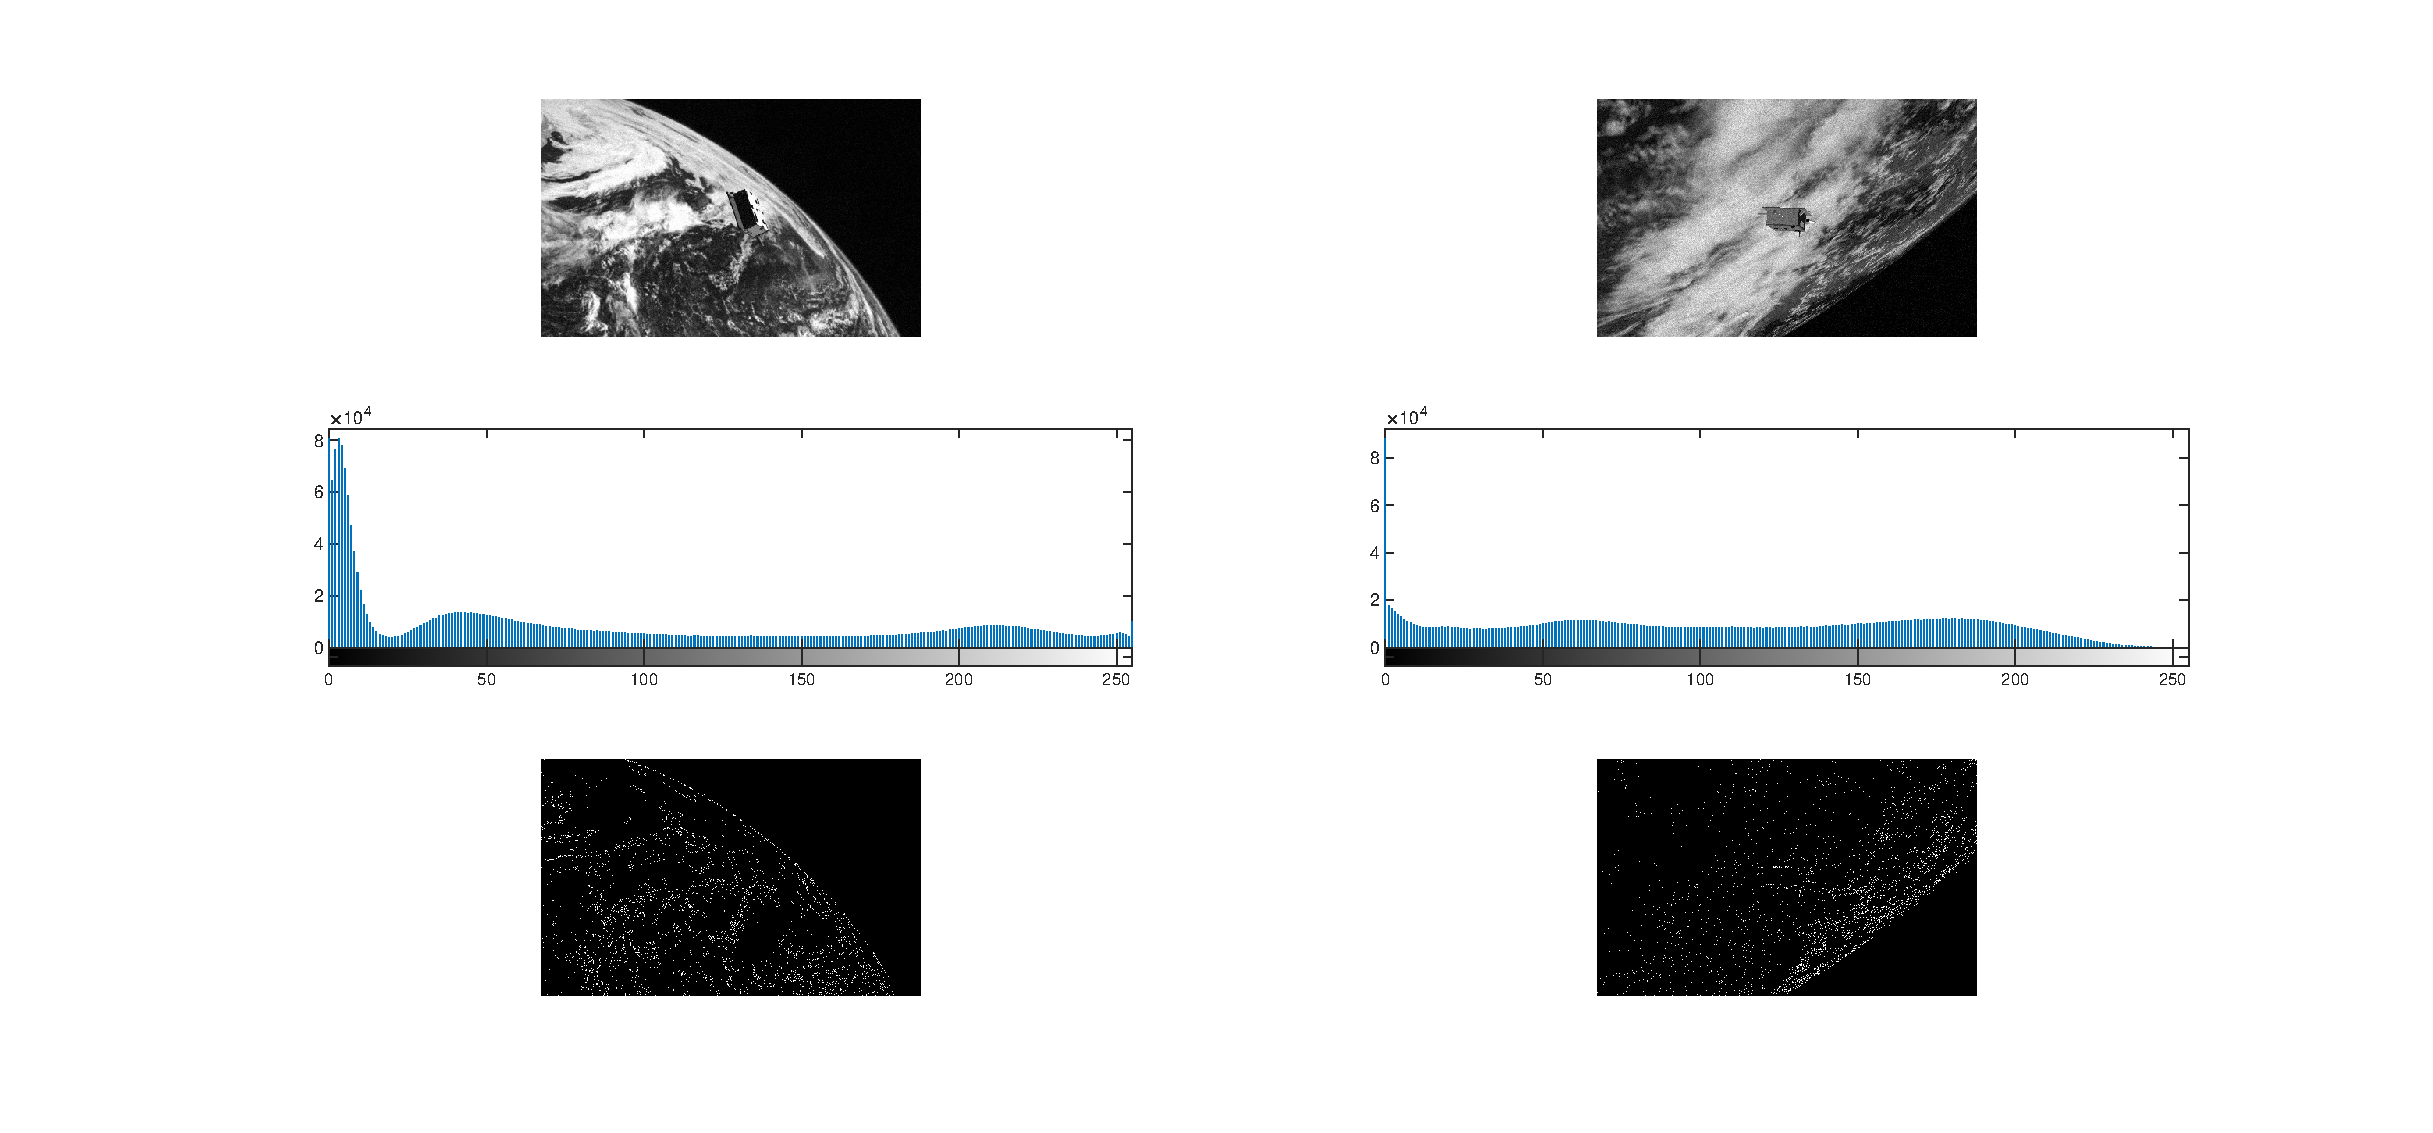
\includegraphics[width=1.0\textwidth]{gfx/comparison/comparison4.eps}
  \caption{Comparison between the SPEED data-set (left) and images generated using the toolbox presented in chapter \ref{chap:second-chapter} (right), 4}
  \label{fig:comparison4}
\end{figure}

In figures \ref{fig:comparison1}, \ref{fig:comparison2}, \ref{fig:comparison3} are presented three simulated images of the Tango \acrshort{sc} on a black background.
Overall, it is possible to recognize that the images belonging to the SPEED shows a better representation of the external look of the \acrshort{sc}, for both the solar panels and the external appendages and external structures. Usually, for rendering images of \acrshort{sc}s, the manufacturer makes available textures of the external look of the whole \acrshort{sc}. For this project unfortunately, due to the unavailability of said textures, the whole look of had to be recreated by hand, doing several experiments and comparisons. This is particularly visible when looking at solar panels, where the SPEED images are of an order of magnitude superior in terms of accuracy and realness of what is being represented.
Despite said issues however, by looking at the forms of the histograms it is possible to recognize that histograms belonging to the SPEED images and histograms belonging to the images used though this project are essentially similar. They both shows the same exponential behavior. The images belonging to the SPEED data-set shows an overall greater concentration of dark values with respect to the ones generated with the toolbox presented in chapter \ref{chap:second-chapter}. This is likely to be due to slightly different scenes being represented in terms of illumination conditions and shadows.
The Sobel edge images are also very similar. The images generated for this project presents a slightly higher level of noise (recognizable by the more presence of little white pixels). This can be due to a different $\sigma^2$ value used to add Gaussian white noise to the image during the post-processing phase.
Lastly, in figure \ref{fig:comparison4} is showed a comparison were the Earth is in the background. As it can be clearly seen by the reader, the Earth is represented more accurately in the SPEED data-set, but this is simply due to the fact that for the SPEED data-set the Earth images comes from actually real space imagery. As described in \cite{Sharma2019}, the Earth images used for the SPEED data-set are composed by 72 actual images of the Earth captured by the Himawari-8 geostationary meteorological satellite. The 72 images each provide a \num{100e6} pixels resolution disk-view of the Earth and were taken 10 minutes apart from each other over a period of 12 hours. The quality the Earth has in the images generated with the toolbox developed during this work can be enhanced by using a texture with an higher resolution, however this comes at the cost of long rendering times and greater RAM usage for rendering the single image. Generating one single image where the Earth is present in the background takes approximately \SI{3}{\s} and occupy \textit{circa} $2$ Gb of RAM on an Intel Core i7-4500U CPU when using mercator images rescaled to $21600 \times 10800$ pixel resolution. Better results can be archived using the full $43200 \times 21600$ pixel original mercator images but rendering times as well as RAM usage would grow too much for the generation of a data-set of hundreds of images on the previously mentioned H/W.

\section{\acrshort{svd} architecture validation}
A further validation of the generated data-set can be obtained by analyzing the synthetic images using a \acrshort{cv} algorithm. In fact, if the quality of the generated images is poor, where for poor it is intended not being photorealistic, the \acrshort{cv} algorithm will not work consistently. Among all state-of-the-art \acrshort{cv} algorithms available, the \acrshort{svd} algorithm has been selected because of its simplicity and effectiveness. In the following sections the most meaningful results will be presented.

\subsection{\acrshort{roi} detection}
The identification of a correct \acrshort{roi} is of vital importance since the edge detection process as well as the merging edges block depends on geometrical parameters which are set as multiplicative constants of the diagonal length of the \acrshort{roi}.

\subsection{Edge detection}

\subsection{Accuracy}